\documentclass[11pt, a4paper]{report}

\usepackage[utf8]{inputenc}
\usepackage[T1]{fontenc}
\usepackage{lmodern}
\usepackage{mathpazo} % Palatino font for a professional look
\usepackage[margin=1in]{geometry}
\usepackage{graphicx}
\usepackage{float}
\usepackage{caption}
\usepackage{subcaption}
\usepackage{booktabs}
\usepackage{hyperref}
\usepackage{amsmath, amssymb}
\usepackage{listings}
\usepackage{xcolor}
\usepackage{titling}
\usepackage{titlesec}
\usepackage{parskip}
\usepackage{longtable}
\usepackage{tikz}
\usepackage{pdfpages}
\usetikzlibrary{shapes,arrows,positioning,calc,fit}

% Colors setup for code listings
\definecolor{codegreen}{rgb}{0,0.6,0}
\definecolor{codegray}{rgb}{0.5,0.5,0.5}
\definecolor{codepurple}{rgb}{0.58,0,0.82}
\definecolor{backcolour}{rgb}{0.95,0.95,0.92}
\definecolor{maroon}{rgb}{0.6,0.13,0.26}

\lstdefinestyle{mystyle}{
    backgroundcolor=\color{backcolour},   
    commentstyle=\color{codegreen},
    keywordstyle=\color{magenta},
    numberstyle=\tiny\color{codegray},
    stringstyle=\color{codepurple},
    basicstyle=\ttfamily\footnotesize,
    breakatwhitespace=false,         
    breaklines=true,                 
    captionpos=b,                    
    keepspaces=true,                 
    numbers=left,                    
    numbersep=5pt,                  
    showspaces=false,                
    showstringspaces=false,
    showtabs=false,                  
    tabsize=2
}
\lstset{style=mystyle}

% Link colors
\hypersetup{
    colorlinks=true,
    linkcolor=maroon,
    filecolor=magenta,      
    urlcolor=blue,
    pdftitle={WeddingBudget.ai Exhaustive Project Report},
}

\titleformat{\chapter}[display]
  {\normalfont\bfseries\Huge}
  {\filleft\Large\chaptertitlename\ \thechapter}
  {4ex}
  {\titlerule\vspace{2ex}\filcenter}
  [\vspace{2ex}\titlerule]

% Provide a flexible graphics path
\graphicspath{{../assets/}{./assets/}{assets/}}

\title{
    \textbf{\Huge WeddingBudget.ai}\\[1em]
    \Large An Autonomous Multi-Agent System for AI-Powered\\Indian Wedding Budget Estimation and Vendor Discovery\\[2em]
    \large \textit{Project Documentation \& Technical Report}
}
\author{Team: 404 Dulhan Not Found}
\date{March 2026}

\begin{document}

\maketitle

\begin{abstract}
Planning an Indian wedding is a logistically complex and financially opaque process. The variance in vendor pricing, specifically across different cities and subjective aesthetic categories such as décor, poses a significant problem for couples attempting to ascertain a realistic budget. This report details the architecture, design, and implementation of \textbf{WeddingBudget.ai}, a full-stack, AI-powered estimation platform. By unifying deterministic rule-based modeling with a subjective Neural Network regression pipeline initialized by CLIP embeddings, the system generates comprehensive Low, Mid, and High cost estimations in under 90 seconds. The backend is powered by a concurrent, 7-agent orchestrator streaming progress over WebSockets. Additionally, this report covers the robust data scraping pipeline required to bypass the lack of localized datasets, the open-source integration of Geo-spatial features via OpenStreetMap's Overpass API, and the optimization of a Next.js 15 client architecture delivering a glassmorphism-infused, high-fidelity user interface.
\end{abstract}

\tableofcontents
\newpage

% ------------------------- CHAPTER 1 -------------------------
\chapter{Executive Summary \& Problem Definition}

\section{Introduction}
WeddingBudget.ai represents an intersection between domain-driven financial estimation, distributed web crawling, computer vision, and reactive web architecture. Rather than treating wedding planning as a flat calculation, the system models an event through functional agents, mapping to the real-world responsibilities of dedicated wedding planners. 

\section{The Core Problem}
The average Indian wedding hosts 300 to over 1,000 guests across 5 to 7 ceremonial events (e.g., Mehendi, Sangeet, Haldi, Pheras, Reception). Generating an initial budget to evaluate geographic feasibility (e.g., Udaipur vs. Goa) typically requires 6 to 8 weeks of manual consultations with local agents. Existing online calculators rely on gross generic percentages, lacking situational awareness, guest-level heuristics, or geographic context. Furthermore, subjective categories such as ``décor'' scale non-linearly, rendering standard lookup tables obsolete.

\section{The Proposed Solution}
To bridge this gap, WeddingBudget.ai presents a hyper-localized estimation pipeline driven by a \textbf{7-Agent Swarm}. Five agents handle deterministic features (Venue, Logistics, Artists, F\&B, Sundries), one agent executes Machine Learning regression on subjective variables (Décor), and an asynchronous agent scrapes OpenStreetMap for nearby verified vendors natively utilizing Haversine routing.

% ------------------------- CHAPTER 2 -------------------------
\chapter{System Architecture}

\section{High-Level Topology}
The system bridges a high-performance Next.js React frontend, utilizing Server-Side Rendering (SSR), with a FastAPI asynchronous backend deployed continuously over WebSockets. 

\begin{figure}[H]
    \centering
    % Fallback to a box if image is missing
    \IfFileExists{../assets/high_level.jpg}{
        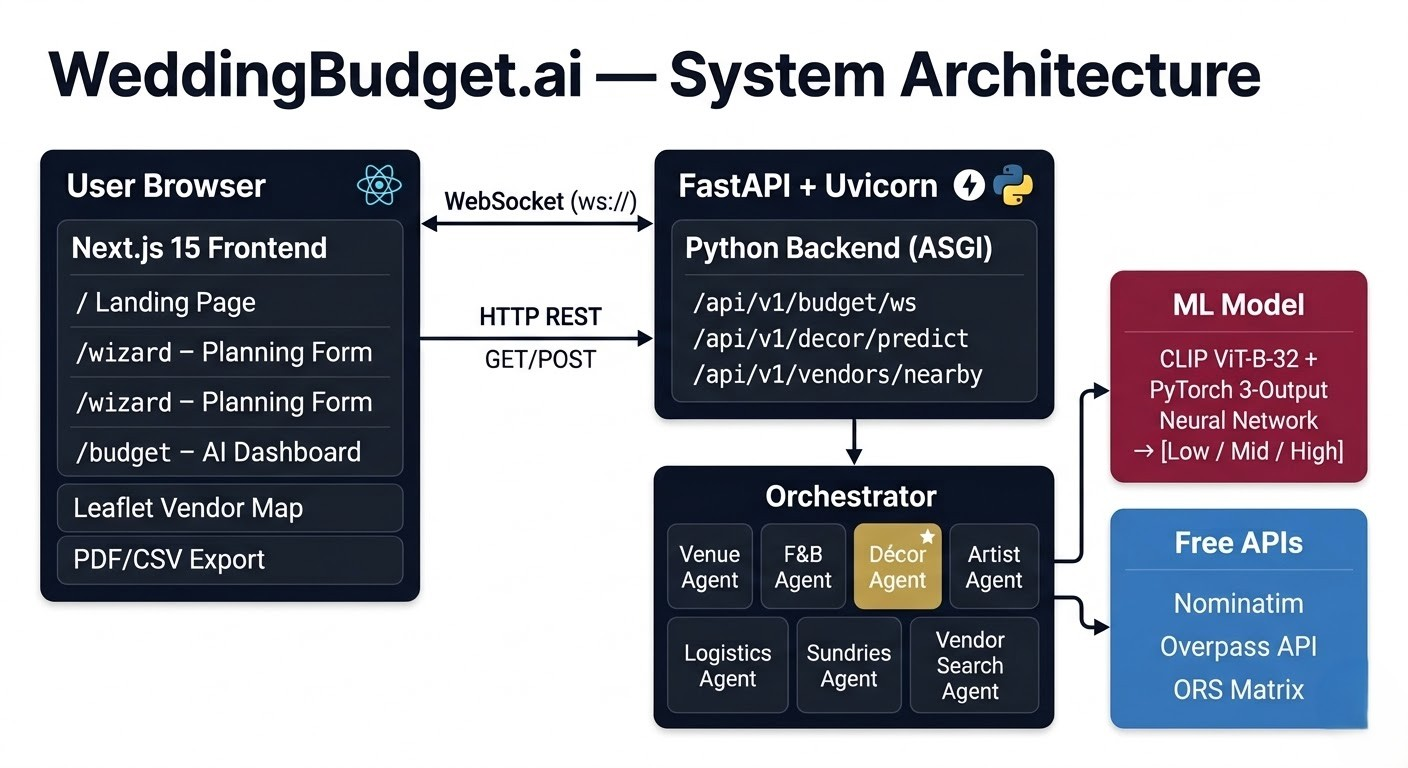
\includegraphics[width=0.9\textwidth]{high_level.jpg}
    }{
        \fbox{\rule{0pt}{3in} \rule{0.9\linewidth}{0pt} \textit{Placeholder: high\_level.jpg}}
    }
    \caption{High-Level System Architecture and Data Flow.}
    \label{fig:high_level}
\end{figure}

The interaction payload begins as a strictly typed JSON object generated by the sequential 6-Step Wizard. The schema dictates strict parameters:
\begin{itemize}
    \item \textbf{City \& Tier:} Drives accommodation multiplication factors.
    \item \textbf{Events Array:} Governs F\&B multiplication limits and DJ/Artist requirement thresholds.
    \item \textbf{Theme \& Complexity:} Extracted and encoded via OpenAI's CLIP model to contextualize visual density.
\end{itemize}

\section{WebSocket Orchestration}
Conventional REST HTTP architectures time out given the theoretical 45-90s resolution time required by the Overpass API and GPU-based PyTorch inference. Therefore, the `/api/v1/budget/ws` endpoint handles the calculation life-cycle. 

The communication protocol leverages strict message types:
\begin{lstlisting}[language=json, caption=WebSocket Message Protocol]
// Server emits progress tick
{ 
    "type": "agent_status", 
    "agent_id": "decor", 
    "status": "working", 
    "message": "Generating embeddings via ViT-B/32..." 
}

// Server returns aggregate completion
{ 
    "type": "final_budget", 
    "total_low": 5200000, 
    "total_mid": 8400000, 
    "categories": [...], 
    "vendors": {...} 
}
\end{lstlisting}

\section{Concurrency Model}
\textbf{Design Decision:} The orchestrator explicitly evaluates agents \textit{sequentially} rather than utilizing \texttt{asyncio.gather()}. 
This deliberate limitation acts as an infrastructural safeguard. The \textit{Vendor Intelligence Module} queries the Overpass API, which implements brutal IP-based rate limiting (HTTP 429). Simultaneously, the Décor Neural Network rapidly reserves VRAM. Sequential operations combined with WebSocket progression simulate real-time computational "thought," sustaining user engagement whilst maintaining memory stability.


% ------------------------- CHAPTER 3 -------------------------
\chapter{Multi-Agent Estimation Pipeline}

The pipeline is governed by a unified \texttt{BaseAgent} abstract class enforcing a standard \texttt{run()} lifecycle emitting execution deltas dynamically. 

\begin{figure}[H]
    \centering
    \IfFileExists{../assets/agent_arch.jpg}{
        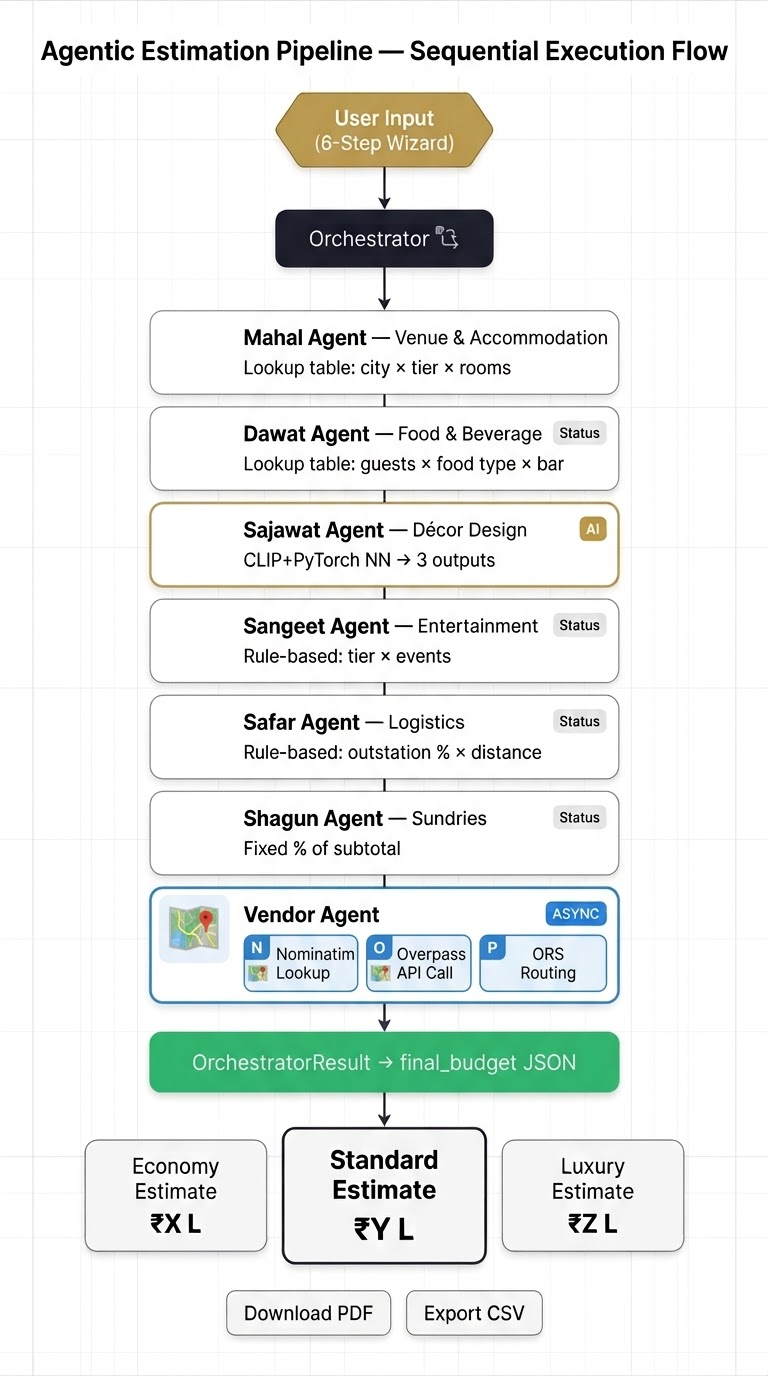
\includegraphics[width=0.8\textwidth]{agent_arch.jpg}
    }{
        \fbox{\rule{0pt}{3in} \rule{0.8\linewidth}{0pt} \textit{Placeholder: agent\_arch.jpg}}
    }
    \caption{UML Abstraction of the BaseAgent Class and Inheriting Swarm.}
    \label{fig:agent_arch}
\end{figure}

\section{Agent Subclasses \& Equations}

\subsection{Mahal Agent (Venue \& Accommodation)}
The backbone of destination weddings. Accommodation is modeled on a \((2.5 \text{ Pax per Room})\) distribution.
\begin{equation}
    Cost = (Rooms_{Req} \times Nights \times Rate(City, Tier)) + (Hall_{Rent})
\end{equation}

\subsection{Dawat Agent (F\&B)}
Models per-plate costing mapped to event density. A "mocktail" multiplier varies drastically from "Full Bar."
\begin{equation}
    Cost = \sum_{e \in Events} (Pax \times PlateRate(City, Tier)) + Bar(Type \times Pax)
\end{equation}

\subsection{Sangeet Agent (Artists \& AV)}
Entertainment requires base infrastructure (Dancefloor, Line Arrays, Truss) plus the performer's fee.
\begin{equation}
    Cost = TierBase(Complexity) \times |Events|
\end{equation}

\subsection{Safar Agent (Logistics \& Travel)}
Models localized airport transfers and vehicle block bookings.
\begin{equation}
    Cost = (Pax \times OutStation \%) \times Transfer(City) + (BlockCars \times Days)
\end{equation}

% ------------------------- CHAPTER 4 -------------------------
\chapter{Machine Learning: Décor Price Estimator}

Unlike venue pricing, event aesthetics possess immense entropy. To address this, the \textbf{Sajawat Agent} intercepts the text description and style complexity, delegating estimation to a custom PyTorch Neural Network.

\section{Network Architecture}
A traditional regression model struggles with categorical sparsity in aesthetics. To provide contextual understanding, the system utilizes \textbf{OpenAI's CLIP (ViT-B/32)} to encode prompt text into a 512-dimensional continuous latent space.

\begin{figure}[H]
    \centering
    \IfFileExists{../assets/ml.jpg}{
        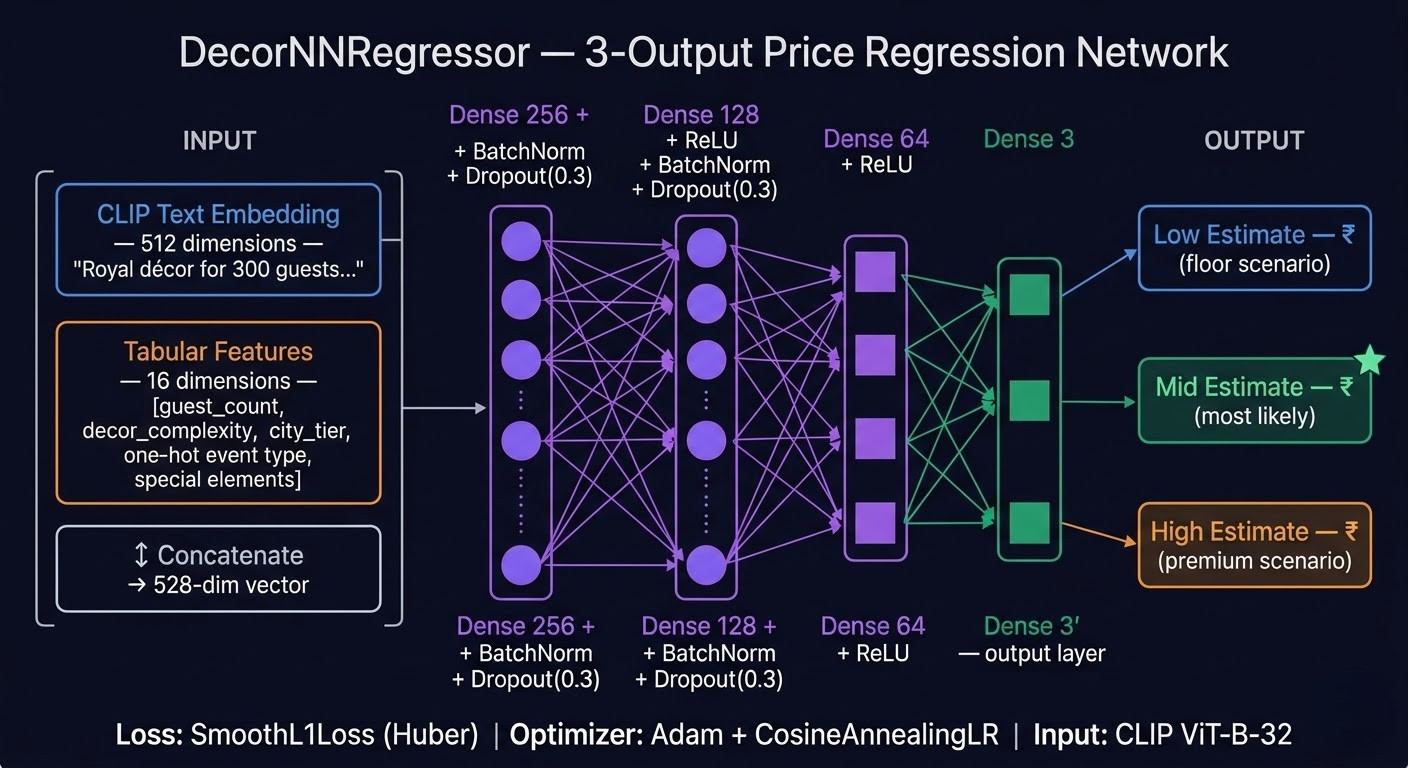
\includegraphics[width=0.9\textwidth]{ml.jpg}
    }{
        \fbox{\rule{0pt}{3in} \rule{0.9\linewidth}{0pt} \textit{Placeholder: ml.jpg}}
    }
    \caption{The Décor Estimation Neural Network.}
    \label{fig:ml_arch}
\end{figure}

The 512-D embedding is concatenated with a 16-D tabular vector specifying deterministic features (Guest Count, City Tier, Outdoor boolean). 
The combined 528-D vector propagates through:
\begin{itemize}
    \item \texttt{Dense(256)} + ReLU + BatchNorm + Dropout(0.3)
    \item \texttt{Dense(128)} + ReLU + BatchNorm + Dropout(0.3)
    \item \texttt{Dense(64)} + ReLU
    \item \texttt{Dense(3)} $\rightarrow$ yielding $[Low, Mid, High]$
\end{itemize}

\section{A Three-Output Paradigm}
Indian market psychology relies on negotiation margins. Providing a single point prediction is inherently flawed. The neural network explicitly trains on three isolated regression targets, outputting a continuous distribution. To suppress sensitivity to erratic outliers in training labels, the network optimizes over \textbf{Huber Loss (Smooth L1 Loss)}:

\begin{equation}
    L_\delta(y, f(x)) = 
    \begin{cases} 
      \frac{1}{2}(y - f(x))^2 & \text{for } |y - f(x)| \le \delta \\
      \delta |y - f(x)| - \frac{1}{2}\delta^2 & \text{otherwise}
    \end{cases}
\end{equation}

% ------------------------- CHAPTER 5 -------------------------
\chapter{Synthetic Data \& Scraping Engineering}

Due to the fundamental lack of open-source datasets pertaining to the Indian Wedding Industry, a custom scraping pipeline was engineered.

\section{Concurrent Sourcing Strategy}
The pipeline targets 15 unique combinations (5 Functions $\times$ 3 Core Styles). To generate critical mass, the system scrapes images across four disparate platforms: Pixabay, Pexels, Unsplash, and Pinterest. 

\begin{figure}[H]
    \centering
    \IfFileExists{../assets/scraping_pipeline.jpg}{
        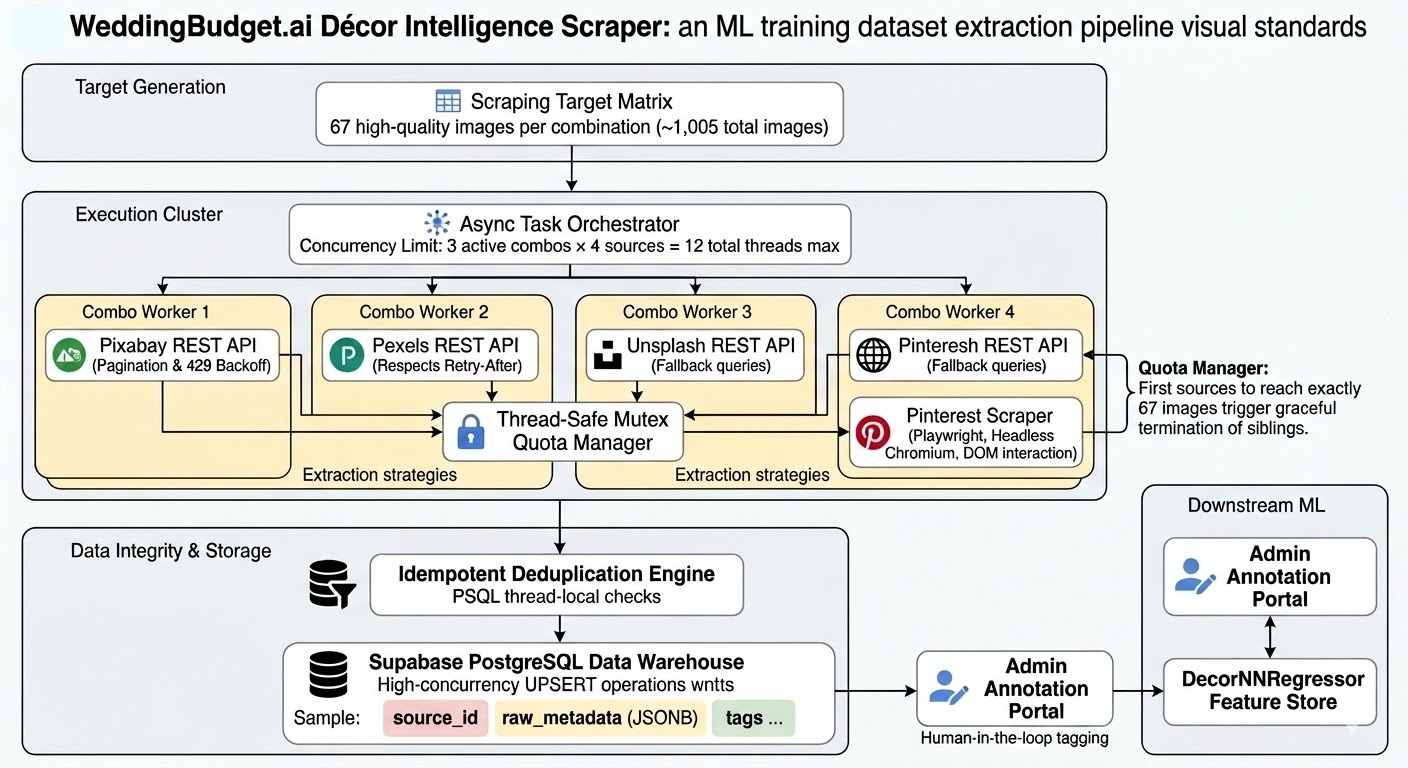
\includegraphics[width=0.85\textwidth]{scraping_pipeline.jpg}
    }{
        \fbox{\rule{0pt}{3in} \rule{0.85\linewidth}{0pt} \textit{Placeholder: scraping\_pipeline.jpg}}
    }
    \caption{Multi-Threaded Concurrent Image Scraping Logic.}
    \label{fig:scraping}
\end{figure}

\section{Thread-Safety and The SharedQuota}
With a target of 67 verified images per combination, independent threads racing towards completion induce fatal over-fetching without synchronization. 

We implemented a Mutex-guarded \texttt{SharedQuota} integer buffer. Across the theoretical maximum of 12 simultaneous HTTP/CrOS headless threads, resource locking guarantees exact volumetric alignment:
\begin{lstlisting}[language=Python]
class SharedQuota:
    def __init__(self, target):
        self._count = 0
        self._lock = threading.Lock()

    def claim(self) -> bool:
        with self._lock:
            if self._count < 67: 
                self._count += 1
                return True
            return False
\end{lstlisting}

This logic ensures that if the Pinterest scraper receives a shadow-ban, the Pixabay thread inherits the remaining computational allocation effortlessly.

\section{Storage and Idempotency}
Records are written into a Supabase PostgreSQL instance under the \texttt{decor\_library} schema. The SQL constraints utilize `ON CONFLICT (source\_id) DO UPDATE` to facilitate repeated cron-job execution without data duplication. Thread-local connection variables eliminate \texttt{psycopg2} pooling crashes.

% ------------------------- CHAPTER 6 -------------------------
\chapter{Vendor Intelligence Module}

Real-world budgets demand real-world suppliers. The \textbf{Nearby Vendor Agent} relies entirely on robust Geographic Information Systems (GIS) without absorbing financial overhead from Google Maps.

\section{Geocoding Pipeline}
\begin{enumerate}
    \item \textbf{Nominatim:} Converts literal string inputs ("Udaipur") to localized $(latitude, longitude)$ tuples.
    \item \textbf{Overpass API:} Utilizes custom Overpass Query Language (OQL) schemas scanning a 20-kilometer radius around the epicenter, searching for nodes tagged with \texttt{amenity=catering}, \texttt{shop=photography}, or \texttt{tourism=hotel}.
    \item \textbf{Fall-back Haversine Routing:} To sort vendors by proximity radially if ORS matrix availability degrades.
\end{enumerate}

\begin{figure}[H]
    \centering
    \IfFileExists{../assets/api.jpg}{
        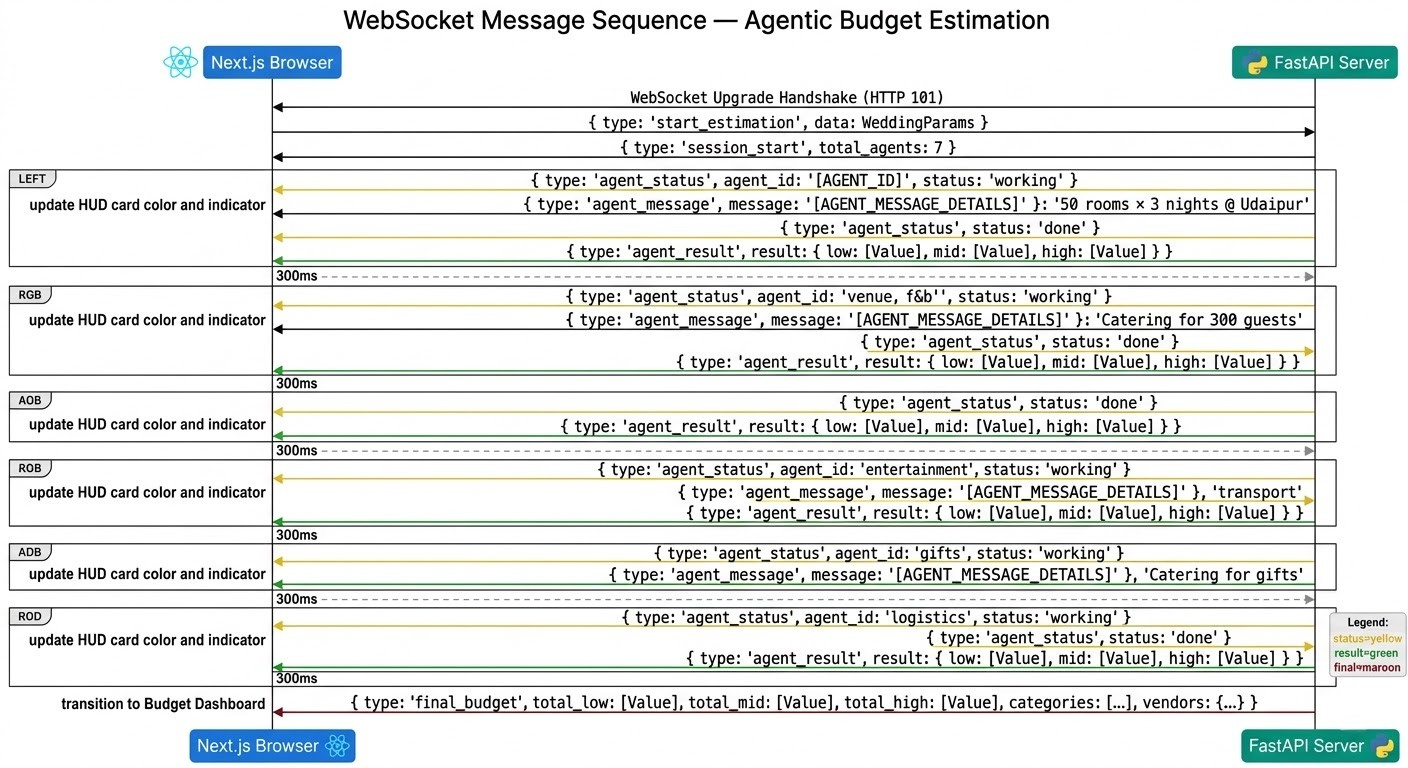
\includegraphics[width=0.7\textwidth]{api.jpg}
    }{
        \fbox{\rule{0pt}{3in} \rule{0.7\linewidth}{0pt} \textit{Placeholder: api.jpg}}
    }
    \caption{API Dependency Chain for OSS Vendor Sourcing.}
\end{figure}

The orchestrator explicitly traps HTML 504 Gateway errors triggered by Overpass servers during heavy OSM community use. A trapped exception yields an empty array to the frontend gracefully, maintaining core budgeting integrity.

% ------------------------- CHAPTER 7 -------------------------
\chapter{Frontend Architecture \& User Interface}

The frontend is built on \textbf{Next.js 15} taking full advantage of the App Router and Turbopack optimizations. 

\section{UI Design System \& Glassmorphism}
The system establishes a premium, authoritative visual identity catering to HNI (High Net Worth Individual) wedding aesthetics.
\begin{itemize}
    \item \textbf{Typography:} \textit{DM Serif Display} enforces editorial luxury, paired with \textit{Inter} for maximal data readability on the HUD.
    \item \textbf{Color Palette:} Dominated by Maroon (\#9A2143), Gold (\#BFA054), and a textured Cream (\#FAF7F2).
\end{itemize}

The Login and Profile layouts leverage advanced CSS \textit{Glassmorphism}. Using gradient positioning overlaid with \texttt{backdrop-filter: blur(8px)}, the UI allows detailed background photography to bleed into structural components without comprising text legibility. Responsive media queries recalculate the focal points for smaller horizontal breakpoints to ensure imagery acts as an interactive hero element on mobile viewports.

\begin{figure}[H]
    \centering
    \IfFileExists{../assets/frontend.jpg}{
        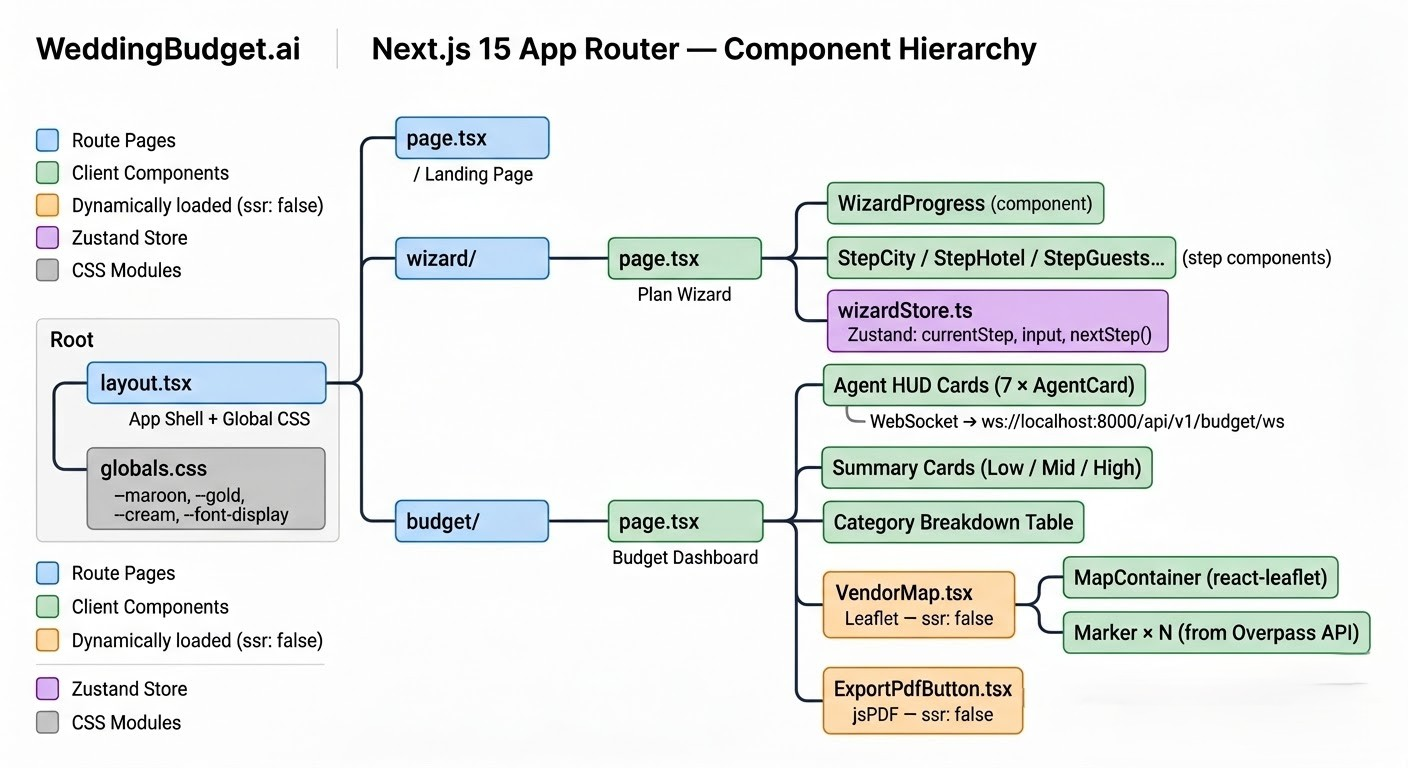
\includegraphics[width=0.8\textwidth]{frontend.jpg}
    }{
        \fbox{\rule{0pt}{3in} \rule{0.8\linewidth}{0pt} \textit{Placeholder: frontend.jpg}}
    }
    \caption{The User Journey Flow Mapping across the Next.js Domain.}
\end{figure}

\section{State Handoff and SSR Strictness}
\textbf{Zustand} governs the volatile 6-step wizard arrays. To facilitate strict decoupled routing, the \texttt{WeddingParams} payload writes to browser \texttt{localStorage} ahead of the push to \texttt{/budget}.

Two key dependencies forcefully mandated \texttt{ssr: false} dynamic imports:
\begin{enumerate}
    \item \texttt{Leaflet.js} manipulates the raw DOM window exclusively. 
    \item \texttt{jsPDF} and \texttt{html2canvas} employ NodeJS internal workers (\texttt{fflate}) which crash server-side pre-compilation on Vercel Edge networks. 
\end{enumerate}
Dynamic encapsulation isolated these elements exclusively to the client-execution tree.

% ------------------------- CHAPTER 8 -------------------------
\chapter{Security, Privacy, and Constraints}

\section{Authentication}
To establish frictionless adoption, the core estimation engine removes authentication boundaries. The system implements isolated \textbf{Firebase Authentication} explicitly for Admin dashboard operations and saved PDF recovery. Place-holder fallback implementations exist to intercept `.env.local` propagation errors intelligently gracefully throwing a browser dialog rather than a fatal Next.js 500 stack trace.

\section{Data Environment}
As operations occur entirely via stateless WebSocket parsing, no User PII is retained in database partitions unless explicitly logged via the PDF backup integration. 
API validation passes through Pydantic validators on the FastAPI router, dropping mismatched schemas intrinsically.

% ------------------------- CHAPTER 9 -------------------------
\chapter{Performance Benchmarks}

Execution metrics collected via localhost and cloud-simulated throttles demonstrate acceptable latency configurations aligning with progress-bar psychological safety metrics.

\begin{table}[H]
    \centering
    \renewcommand{\arraystretch}{1.5}
    \begin{tabular}{@{} l c l @{}}
        \toprule
        \textbf{Operation Segment} & \textbf{Time (Approx)} & \textbf{Primary Bottleneck} \\
        \midrule
        Rule-Based Aggregations (5 Agents) & $2-4$ \text{sec} & Python List Comprehensions \\
        Décor Prediction (CLIP + PyTorch) & $8-15$ \text{sec} & VRAM Latency / CPU Inference Fallback\\
        Vendor Sourcing (Overpass API) & $20-45$ \text{sec} & Nominatim DNS \& OSM Server Load \\
        \midrule
        \textbf{Full Pipeline Resolution} & $\mathbf{45-90}$ \textbf{sec} & \textbf{Synchronous Thread Locking} \\
        \midrule
        Leaflet Maps Hydration & $0.5$ \text{sec} & Tile Server Round-trip \\
        jsPDF Canvas Export & $3-5$ \text{sec} & Client-device DOM parsing \\
        \bottomrule
    \end{tabular}
    \caption{System Performance Profiling}
\end{table}

% ------------------------- CHAPTER 10 -------------------------
\chapter{Future Roadmap \& Conclusion}

WeddingBudget.ai establishes that highly subjective, culturally-nuanced planning estimations can be mechanized dynamically via Large Vision Models and multi-agent coordination.

\section{Roadmap Expansion}
\begin{itemize}
    \item \textbf{Image Prompting:} Enabling brides to upload Pinterest boards directly to the UI. Expanding the semantic CLIP pipeline into direct Image-to-Image similarity parsing.
    \item \textbf{Fine-Tuning Loop:} Establishing Human-in-the-Loop reinforcement arrays whereby finalized vendor invoices correct PyTorch weights over sustained epochs.
    \item \textbf{B2B Ecosystems:} Enabling a SaaS portal for wedding planners to issue branded, modified reports direct to clientele.
\end{itemize}

\section{Conclusion}
By offloading heuristic and analytical computations to distinct agents while preserving statefulness over a high-fidelity Next.js visual layer, this platform mitigates weeks of anxiety for families. It operates cost-effectively via OSM integration and efficiently scales via stateless GPU delegation. 

\vspace{2cm}
\begin{center}
    \Large \textit{Plan smarter. Celebrate bigger. Worry less.}
\end{center}

\end{document}
